%!TEX root=seke.tex
% mainfile: ../seke.tex

According to the decisions produced by the regression tree, the choice of coverage criterion and data generator have an
impact on the runtime of \textit{SchemaAnalyst}. To show the effect of these choices, we present
Figure~\ref{fig:crites}, which shows the effect of coverage criterion on runtime, and Figure~\ref{fig:datas}, which
shows the effect of data generator on runtime.

For coverage criteria, the most apparent pattern is that AUCC, ClauseAICC, and CondAICC seem to cause runtime to
increase by about the same amount, with the other criterions taking roughly the same amount of time.

For data generator, the Random and Random Defaults generators took the most amount of time by a distinctive margin, and
a less pronounced hierarchy between AVM, AVM defaults, Directed Random, and Directed Random Defaults can be observed.


\begin{figure}
\centering
  \centering
  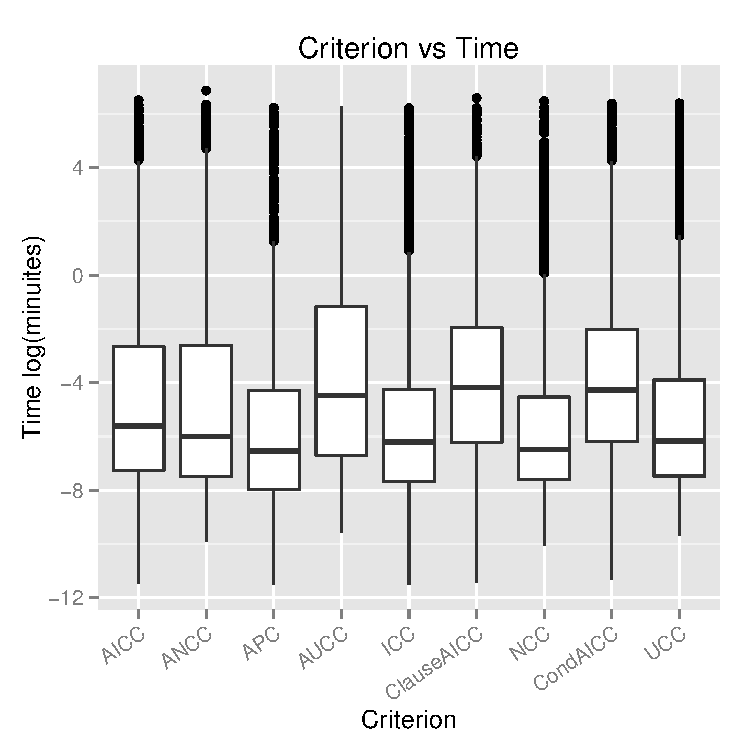
\includegraphics[width=1\linewidth]{diagrams/CriterionvsTime.pdf}
  \caption{Coverage criterion versus runtime in minutes.\vspace{-.15in}}
  \label{fig:crites}
  \vspace{-.15in}
\end{figure}

\begin{figure}
\centering
  \centering
  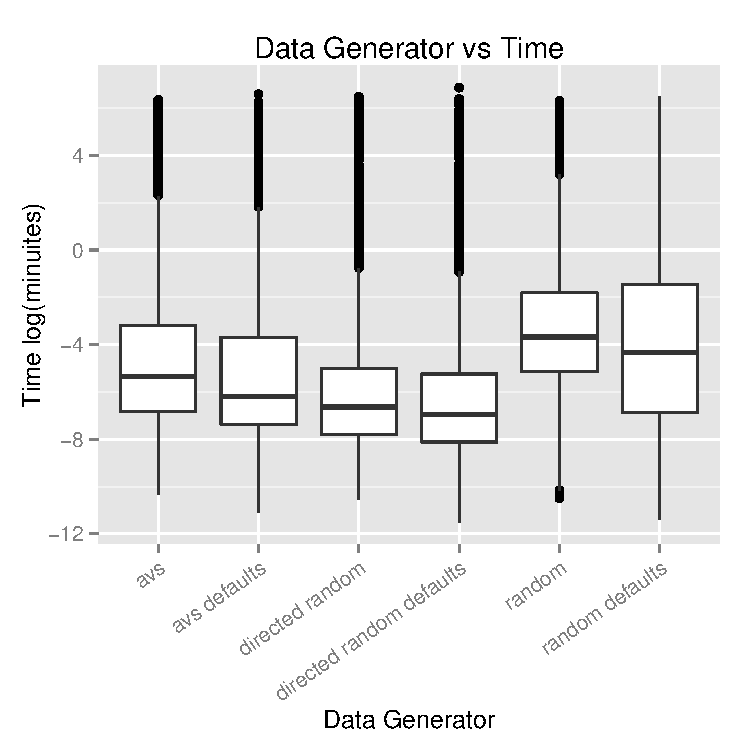
\includegraphics[width=1\linewidth]{diagrams/DataGeneratorvsTime.pdf}
  \caption{Data generator versus runtime in minutes.\vspace{-.15in}}
  \label{fig:datas}
  \vspace{-.15in}
\end{figure}
